Implementation strategies are highly dependant on the programming language and game engine used. It requires good knowledge of both for effective results. One observation done during previous runs is a noticeable improvement in framerates while the shield is down. Because of extensive usage of shader properties and particles, one attempt at optimization will be creating a similar, simpler force field effect, that will be dynamically chosen at runtime, in case of Handheld devices. The choice between the two effects can be done when initializing the game scene, thus having no impact during the actual gameplay, save for the benefits of a simpler effect in case of a handheld device.  \\
Dickinson strongly discourages the usage of Draw Calls on mobile platforms, specifically related to high material counts, as well as alpha testing. It is therefore recommended to reuse as many materials as possible, with preferably square sized, low size textures, which will also improve VRAM and Memory Bandwidth usages. For example, the iPhone 6S could only support texture sizes of up to 2048x2048. \cite{optimizationbook} In Space Shooter, due to the low performing hardware used, all textures will be reduced to 256x256 sizes. This optimization may be considered as fitting under the Quality Comporomises section, but due to the subtlety of knowledge involved, it was decided it fits better here. \\ \\
An additional, minor improvement, is going through each of the scripts, and removing the autogenerated methods. Each class derived from Unity's MonoBehaviour will have a number of callback functions defined empty. At runtime, when the MonoBehaviour class is instantiated, all the implemented methods will be hooked, regardless of it being empty. Some of these functions (such as Update, called every frame, for every object, or OnCollisionEnter, in the presence of a RigidBody) can add an overhead that keeps adding up, slowing down the CPU side of the processing. \cite{optimizationbook} We will attempt at removing and avoiding all unnecessary function definitions, and ensure that actions that only need to be taken once are placed in the right function, for example the dynamic choice of force field effect should be done during the call to Start or Awake, which only execute once, during initialization, instead of the Update function.
Figure 6 shows the results of further optimizing Space Shooter, after the previous section. On the PC, the differences are very subtle. The mean values are so close, 175 to 179, that it could be attributed to background interference. However, a slightly increased mean, and a slightly decreased standard deviation would suggest a minor uniformization of the framerate, which is one of the goals. \\
On the mobile side of things, the results are a little better. The average framerate shows a 35.44\% improvement, with an approximate 130\% increase in standard deviation. While the minimum, maximum and bottom 10 average are mostly unchanged, we can see that along with the higher standard deviation, the top 10 mean is also showing an increase of almost 45\%, suggesting that likely textures were one of the contributing factors. \\ \\
\begin{figure}
\begin{subfigure}{0.49\textwidth}
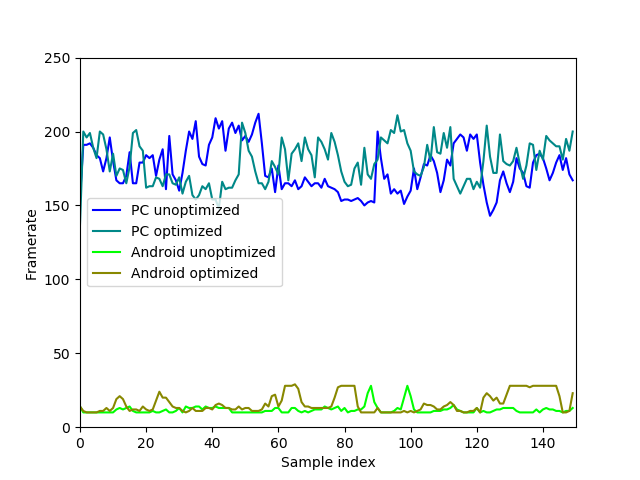
\includegraphics[width = \textwidth, height = 0.66\textwidth]{images/general}
\end{subfigure}
\caption{Framerate before and after optimization}
\end{figure}
\begin{table}
\caption{Optimization data}
\label{tab:conf}
\begin{minipage}{0.49\textwidth}
\begin{center}
\begin{tabular}{lllll}
Value & PC pre & PC post & Android pre & Android post \\
Mean & 175.08 & 178.94 & 11.82 & 16.01 \\
Std & 15.68 & 14.40 & 2.75 & 6.32 \\
Top 10 mean & 205.50 & 203.00 & 19.40 & 28.10 \\
Bottom 10 mean & 150.50 & 153.80 & 10.00 & 10.00 \\
Min & 143 & 137 & 10 & 10 \\
Max & 212 & 211 & 28 & 29 
\end{tabular}
\bigskip
\end{center} 
\end{minipage}
\end{table}
While we have seen no dramatic increase in numbers with any of the optimizations so far, comparing Figures 5 and 6, we have improved the performance of the game by around 50\%. Ideally, the numbers can be pushed higher by further optimizations, and reaching the goal of a stable framerate, averaging at least 24 frames per second, the minimum value for an animated experience, preferably with a small deviation for consistency. \cite{fpspaper}